\documentclass{beamer}
 
\usepackage[utf8]{inputenc}
\usepackage{tkz-euclide} 
\usetkzobj{all}
 
\title{package Tkz-euclide}
\author{Jakub Karmański}
\institute{POLSL RMS rok III sem.V}
\date{2019}
 
 
 
\begin{document}
\frame{\titlepage}
 
\begin{frame}
\frametitle{ZAD 1}

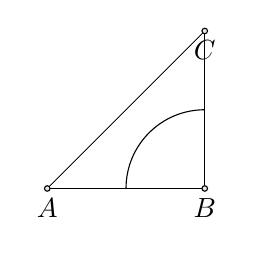
\begin{tikzpicture}[scale=1] 
\tkzDefPoints{0/0/A,2/0/B,2/2/C} 
\tkzDrawSegments(C,A A,B B,C C,A) 
\tkzDrawPoints(A,B,C) 
\tkzLabelPoints(A,B,C) 
\tkzDefCircle[in](A,B,C) 
\tkzMarkAngles(C,B,A)
\end{tikzpicture}
 
 
\end{frame}

\begin{frame}
\frametitle{ZAD 2}

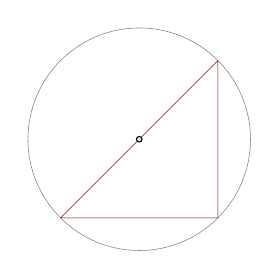
\begin{tikzpicture}
\tkzDefPoints{0/0/A,2/0/B,2/2/C} 
\tkzDrawPolygon[color=Maroon](A,B,C)
\tkzCircumCenter(A,B,C)
\tkzGetPoint{G}
\tkzDrawPoint(G)
\tkzDrawCircle(G,A)
\end{tikzpicture}

\end{frame}

\begin{frame}
\frametitle{ZAD 3}

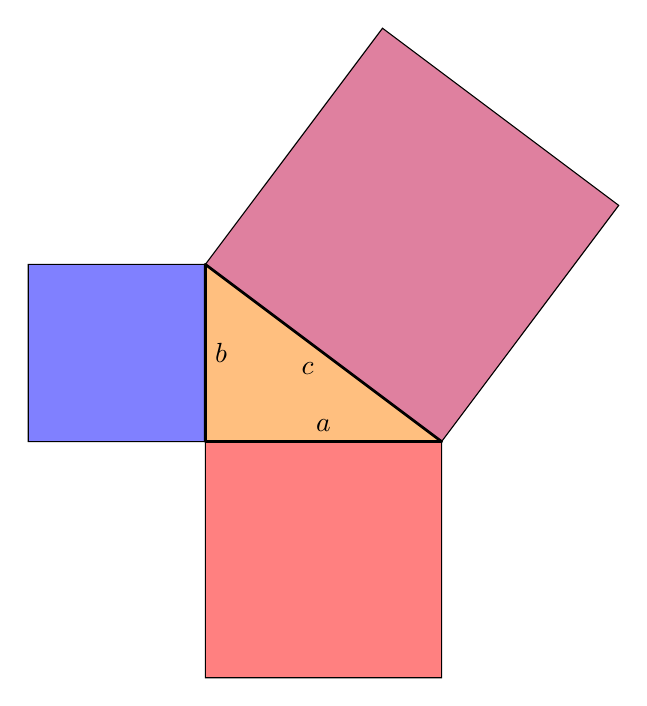
\begin{tikzpicture}[scale=.75]
\tkzInit[xmax=5,ymax=5]
\tkzDefPoint(0,0){C}
\tkzDefPoint(4,0){A}
\tkzDefPoint(0,3){B}
\tkzDefSquare(B,A)\tkzGetPoints{E}{F}
\tkzDefSquare(A,C)\tkzGetPoints{G}{H}
\tkzDefSquare(C,B)\tkzGetPoints{I}{J}
\tkzFillPolygon[draw,
fill = red!50 ](A,C,G,H)
\tkzFillPolygon[draw,
fill = blue!50 ](C,B,I,J)
\tkzFillPolygon[draw,
fill = purple!50](B,A,E,F)
\tkzFillPolygon[draw,opacity=.5,
fill = orange](A,B,C)
\tkzDrawPolygon[line width = 1pt](A,B,C)
\tkzLabelSegment[above](C,A){$a$}
\tkzLabelSegment[right](B,C){$b$}
\tkzLabelSegment[below left](B,A){$c$}
\end{tikzpicture}

\end{frame}
 
\end{document}